\chapter{Realizace}

\section{Prostředí}

Popsané algoritmy jsme implementovali v jazyce C99[todo: zdroj]. Implementace probíhala v operačním systému Lubuntu[todo: zdroj], v IDE Eclipse CDT[todo: zdroj]. Zdrojový kód byl kompilován pomocí překladače GNU C[todo: zdroj], s optimalizačním přepínačem \texttt{--Ofast}.

K lazení chyb pro práci s pamětí jsme použili nástroj Valgrind[todo: zdroj] s přepínači \texttt{----leak--check=full ----show-reachable=yes}. Běžící program jsme krokovali pomocí nástroje GNU Debugger[todo: zdroj]. Zdrojový kód pro lazení chyb byl kompilován s přepínači \texttt{--Wall --pedantic --Og --ggdb}.

%-----------------------------------------------------------------------------

\section{Design implementace}

Protože matice mají některé vlastnosti stejné a lze s podobně pracovat, byl zvolen jednoduchý objektově orientovaný model \cite{schreiner1994objektorientierte}. Nadřazeným objektem je virtuální matice \texttt{vm\_t}, obsahující virtuální tabulku funkcí. Obrázek \ref{fig:uml} ukazuje jednoduchý návrh tříd v UML.
	
\begin{figure}[htb]
	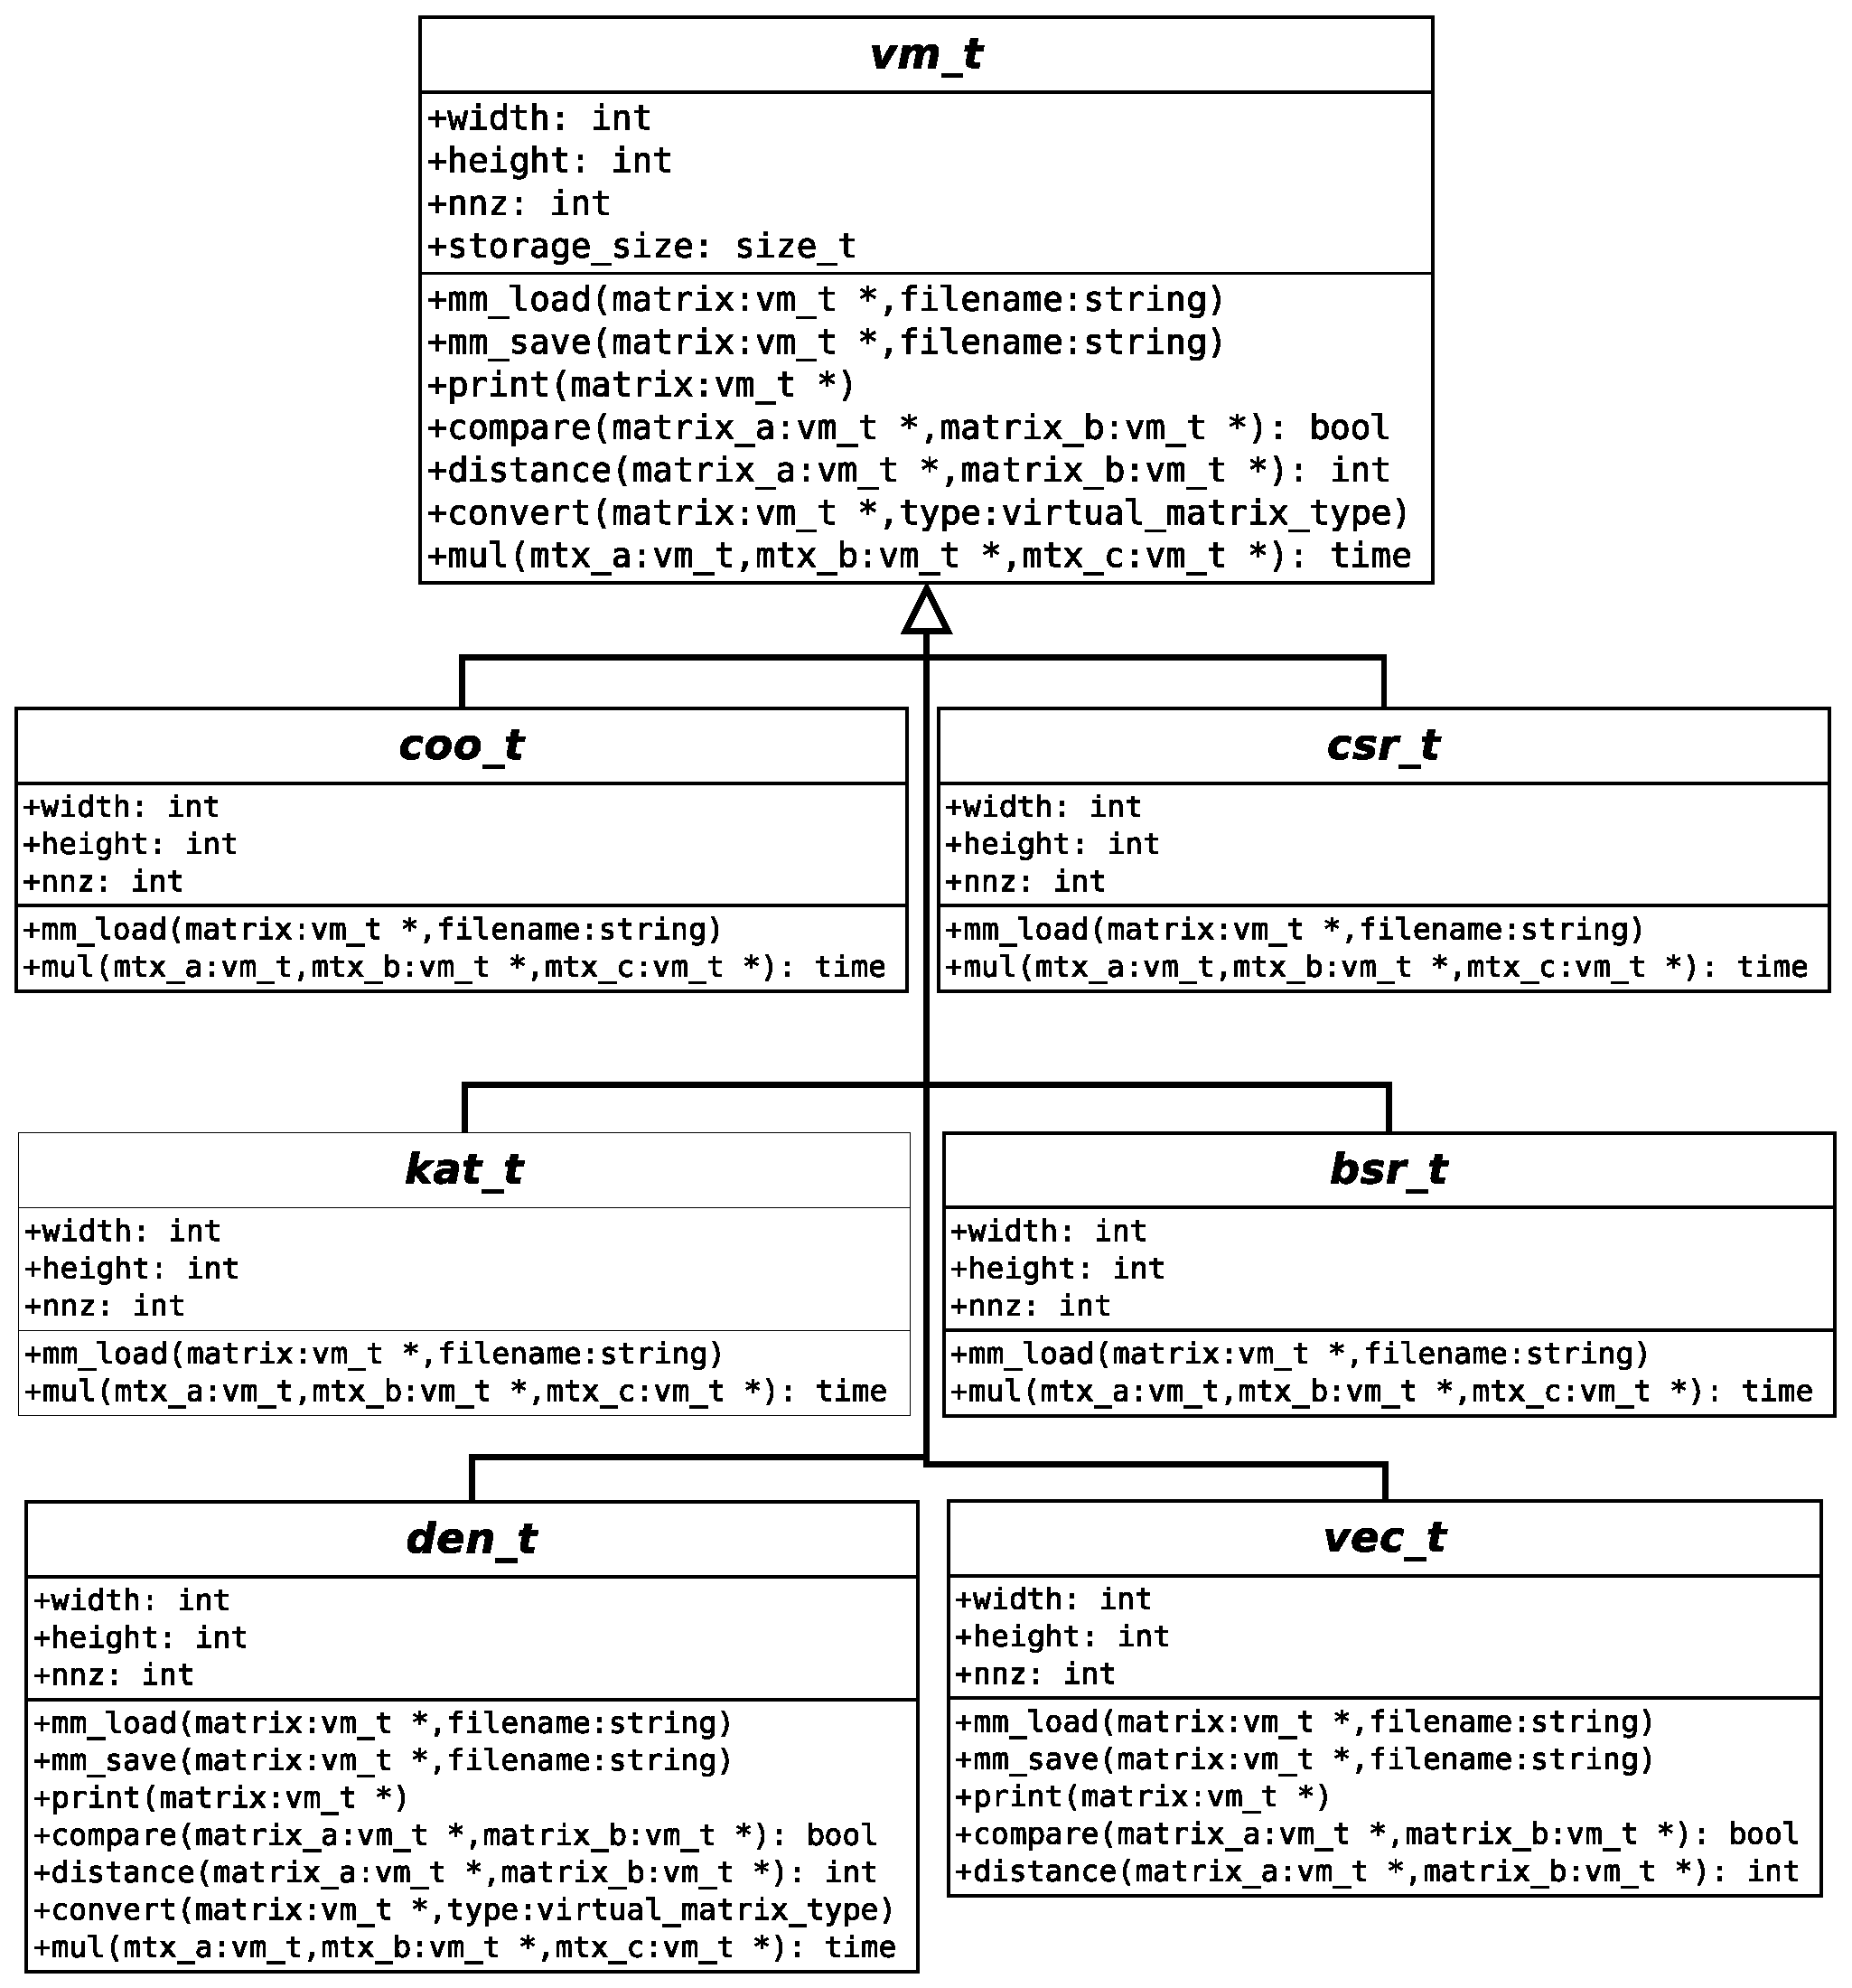
\includegraphics[width=1.0\textwidth]{./images/uml/uml}
	\caption{UML diagram tříd programu}
	\label{fig:uml}
\end{figure}

Program běží v příkazovém řádku bez GUI. Program načte jednu, nebo dvě matice v určitém formátu a vynásobí je. Pomocí přepínačů lze zobrazit, nebo uložit výslednou matici, popřípadě vypsat některé údaje o načtených maticích. Podrobnější popis nastavení programu je v příloze.

%-----------------------------------------------------------------------------

\section{Implementace KAT}

U formátů COO, CSR, BSR je implementace přímočará podle pseudokódů. U implementace KAT máme více možností, proto zde popíšeme naší implementaci.

Jeden z důležitých parametrů je $k$, tedy maximální počet synů vnitřních uzlů. V naší implementaci je tento parametr uložen v konstantě \texttt{KAT.n}, pro připomenutí $KAT.n = sqrt(k)$. Překladač poté cykly, kde iterujeme do této konstanty, rozbalí. Překladači i explicitně sdělujeme, ať cykly rozbalí přes atribut \texttt{\_\_attribute\_\_((optimize("unroll-loops")))}.

V bakalářské práci Rozšíření implementace formátu kvadrantového stromu od Tomáše Karabely[todo: zdroj] je Quadtree implementován jako strom, jehož listy tvoří virtuální matice podobným těm v naší práci. Protože jeho formát byl určený pro algoritmus LU rozklad, jeho virtuální matice musely umět přijímat i další prvky. Protože v naší práci se s formáty uložení řídké matice zachází jako s konstantami, rozhodli jsme se hodnoty prvků a informace v polích \texttt{row\_pointers} a \texttt{col\_indices} uložit mimo listy stromu. V listech se nachází ukazatel do velkého pole na příslušné místo pro daný list. Ušetříme tak práci knihovně libc s mnohonásobným volání funkce \texttt{malloc}

\subsection{Tvoření stromu}

Při tvoření matice v KAT formátu, pro každý prvek procházíme strom a hledáme správný list. Protože výška stromu je daná třemi parametry, tedy velikostí matice $n$, velikostí podmatice $sm\_size$ a počtu větvení uzlu $k$, nejefektivnější využití bude, pokud je $n$ bezezbytku dělitelné $k * sm\_size$. Pokud toto neplatí, rodiče listů budou mít část synů nevyužitých i při uložení husté matice. Protože se prvky do matice načítají po řádcích zleva doprava, je velká pravděpodobnost, že další načtený prvek bude patřit do stejného listu. Z tohoto důvodu si pamatujeme poslední list a pokud prvek patří do něj, vrátíme jej. Algoritmus \ref{kat-create} ukazuje, jakým způsobem vyhledáváme list pro prvek.


\label{alg:kat-create}
\begin{algorithm}[htb]
	\caption{Vyhledání listu pro KAT matici}\label{kat-create}
	\begin{algorithmic}[1]
		\Procedure{KAT-getNode}{KAT, y, x}
		\If{ \{y, x\} $\in$ lastLeaf.area}
			\State \texttt{return lastLeaf;}
		\EndIf
		\State \texttt{tmpNode $\gets$ KAT.root;}
		\State \texttt{blockY $\gets$ 0;}\Comment{výřez matice}
		\State \texttt{blockX $\gets$ 0;}
		\State \texttt{blockS $\gets$ KAT.sm\_size;}
		\\\Comment{až do předposledního vnitřního uzlu traverzujeme podle velikosti KAT.n}
		\While{\texttt{blockS > (KAT.n * KAT.sm\_size)}}
			\State \texttt{nodeY $\gets$ (y - blockY) / (blockS / KAT.n);}
			\State \texttt{nodeX $\gets$ (x - blockX) / (blockS / KAT.n);}
			\State \texttt{tmpNode $\gets$ tmpNode.childs[nodeY][nodeX];}
			\State \texttt{blockY += nodeY * (blockS / KAT.n);}
			\State \texttt{blockX += nodeX * (blockS / KAT.n);}
			\State \texttt{blockS /= KAT.n;}
		\EndWhile
		\\\Comment{do posledního vnitnřního uzlu traverzujeme podle velikosti KAT.sm\_size}
		\State \texttt{nodeY $\gets$ (y - blockY) / KAT.sm\_size;}
		\State \texttt{nodeX $\gets$ (x - blockX) / KAT.sm\_size;}
		\State \texttt{tmpNode $\gets$ tmpNode.childs[nodeY][nodeX];} 	
		\\\Comment{nyní je tmpNode list}
		\State \texttt{tmpNode.y $\gets$ $\lfloor$y / KAT.sm\_size$\rfloor$ * KAT.sm\_size ;}
		\State \texttt{tmpNode.x $\gets$ $\lfloor$x / KAT.sm\_size$\rfloor$ * KAT.sm\_size ;}
		\State \texttt{lastLeaf $\gets$ tmpNode;}
		\State \texttt{return tmpNode;}
		\EndProcedure
	\end{algorithmic}
\end{algorithm}

\subsection{Násobení listů matice KAT}

Protože dovolujeme dva druhy listů, tedy hustý a řídký ve formátu CSR, bylo potřeba implementovat následující algoritmy:

\begin{enumerate}
  \item hustý list $\cdot$ hustý list
  \item hustý list $\cdot$ CSR list
  \item hustý list $\cdot$ vektor
  \item CSR list $\cdot$ hustý list
  \item CSR list $\cdot$ CSR list
  \item CSR list $\cdot$ vektor
\end{enumerate}

Protože tyto algoritmy jsou velice podobné již popsaným algoritmům \ref{algo}, ukážeme zde pouze násobení CSR listu s hustým listem.

\begin{algorithm}[htb]
	\caption{Násobení hustého KAT listu s CSR listem}\label{kat-mmm-den-csr}
	\begin{algorithmic}[1]
		\Procedure{KAT-MMM-DEN-CSR}{ka,kb,na,nb,c}\Comment{ka,kb=KAT matice; na,nb=listy, c = hustá matice}
		\For{\texttt{i $\gets$ 0 \TO ka.sm\_size}}
			\For{\texttt{j $\gets$ na.rp[i]\TO na.rp[i]}}
				\For{\texttt{k $\gets$ 0 \TO ka.sm\_size}}
					\State \texttt{C.v[na.y + i][nb.x + k] += na.v[j] * nb.v[ka.sm\_size * na.ci[j] + j];}
				\EndFor
			\EndFor
		\EndFor
		\EndProcedure
	\end{algorithmic}
\end{algorithm}


%-----------------------------------------------------------------------------

\section{Testování}

Pro ověření správnosti algoritmů je potřeba testovací software. Strategie testování v našem programu spočívá ve výběru testovacích matic, vynásobení v hustém formátu uložení, vynásobení v některém z řídkých formátů uložení a porovnaní výsledků.

\begin{algorithm}[htb]
	\caption{Testování}\label{testing}
	\begin{algorithmic}[1]
		\Procedure{\texttt{TestFormats}}{\texttt{PairList, FormatList}}
		\ForAll{\texttt{pair $\in$ PairList}}
				\State \texttt{denseA $\gets$ vm\_load(pair.a, DENSE);}
				\State \texttt{denseB $\gets$ vm\_load(pair.b, DENSE);}
				\State \texttt{denseC $\gets$ vm\_mul(denseA, denseB, denseC);}
			\ForAll{\texttt{format $\in$ FormatList}}		
				\State \texttt{sparseA $\gets$ vm\_load(pair.a, format);}
				\State \texttt{sparseB $\gets$ vm\_load(pair.b, format);}
				\State \texttt{sparseC $\gets$ vm\_mul(sparseA, sparseB, sparseC);}
				\If{ \texttt{vm\_compare(denseC, sparseC) = NOT\_SAME}}
					\State \texttt{print("Error:", pair.a, pair.b, format);}
				\EndIf
			\EndFor
		\EndFor
		\EndProcedure
	\end{algorithmic}
\end{algorithm}

Pro přehled o nefungujících konfiguracích jsme použili testovací framework Cassertion [todo: zdroj].

Při testování jsme i na relativně malých maticích narazili na problém s numerickou stabilitou. Část z testovacích matic má velký desetinný rozvoj a protože čísla jsou v různých formátech násobena v jiném pořadí, dochází k rozdílu mezi výsledky. Při kompilaci programu lze nastavit přesnost výpočtu pomocí typu proměnné pro uchovaní hodnot buď na \texttt{float}, \texttt{double} nebo \texttt{long double}. Při porovnávání dvou matic neporovnáváme hodnoty přímo, ale sledujeme velikost jejich rozdíl. V defaultní konfiguraci je povolená odchylka 0.001, při kompilaci lze změnit. Pokud spustíme testy  pouze s přesností \texttt{float}, část testů selže právě kvůli numerické stabilitě. 

%-----------------------------------------------------------------------------

\section{MatrixMarket}
\label{MM}

MatrixMarket \cite{Boisvert:1997:MMW:265834.265854} je internetová sada matic s vlastním formátem pro uložení řídkých matic \texttt{.mtx}. Tato sada obsahuje skoro pět set matic z různých oblastí. Obsahuje i generátory řídkých matic, jejichž výstupy jsou matice různých vlastností.

Pro náš program jsme zvolili právě formát \texttt{.mtx}. Podporujeme více druhů tohoto formátu. Nesymetrický, s banerem \texttt{\%\%MatrixMarket matrix coordinate real symmetric} a symetrický s banerem \texttt{\%\%MatrixMarket matrix coordinate real general}. Místo reálných čísel podporujeme i druh \texttt{pattern}, kdy nenulové prvky nabývají pouze hodnoty jedna.

Přestože náš program neumí pracovat s komprimovanými soubory, v prostředí unixového systému předáváme programu pojmenovanou rouru do které komprimovanou matici rozbalujeme příkazem \texttt{ <(gzip -cd matrix.mtx.gz) }.

\subsection{Generátor řídkých matic}

Generátory z MatrixMarketu běží v internetovém prohlížeči a v jazyce Java. Protože takto není jednoduché matice generovat ve skriptu, abychom při distribuci našeho programu nemuseli přikládat velké testovací matice, implementovali jsme jednoduchý generátor řídkých matic. Parametry předáváme programu informace o výsledné matici a seznam objektů, tedy buď podmatic nebo diagonál, které mají být do matice zahrnuty. Manuál ke generátoru je možné vypsat zavoláním \texttt{./tests/bin/matrix\_generator -h}.    

\begin{algorithm}[htb]
	\caption{Generování řídkých matic}\label{mmm-recursive}
	\begin{algorithmic}[1]
		\Procedure{SparseMatrixGenerator}{$file,width,height,ItemList$}
		\State \texttt{$MtxWrapper \gets InitMtxWrapper();$}
		\State \texttt{$MtxWrapper.PositionVector \gets InitVector();$}	
		\ForAll{\texttt{$Item \in ItemList$}}
			\State \texttt{$MtxWrapper.addItem(Item.y, Item.x, Item.properties);$}
			\If{$Item.type == Mirrored$}
				\State \texttt{$MtxWrapper.addItem(Item.x, Item.y, Item.properties);$}
			\EndIf
		\EndFor
		\State \texttt{$MtxWrapper.PositionVector.sort();$}
		\State \texttt{$MtxWrapper.PositionVector.removeDuplicates();$}
		\State \texttt{$MtxWrapper.write(file);$}
		\EndProcedure
	\end{algorithmic}
\end{algorithm}

% Generátor řídkých matic byl implementován v jednom souboru. Lze spouštět s následujícími parametry:

% \begin{itemize}
% 	\item \texttt{-c} matice bude obsahovat hlavní diagonálu
% 	\item \texttt{-H <celé číslo>} výška matice
% 	\item \texttt{-i <typ,a,b,c,d,...>} seznam objektů, které se do matice přidají
% 	\begin{itemize}
% 	\item \texttt{diagonal,ay,ax,by,bx,sparsity} prvky v přímce od bodu \texttt{[ax,ay]} do bodu \texttt{[bx,by]} s řídkostí % \texttt{sparsity}
% 	\item \texttt{block,ay,ax,by,bx,sparsity} blok prvků v obdelníku ohraničiného body \texttt{[ax,ay]} a \texttt{[bx,by]} s % řídkostí \texttt{sparsity}
% 	\end{itemize}
% 	\item \texttt{-n <celé číslo>} velikost matice
% 	\item \texttt{-o <soubor>} cílový soubor (lze použít i stdout)
% 	\item \texttt{-s <desetinné číslo>} řídkost matice (\texttt{sparsity})
% 	\item \texttt{-S <desetine číslo>} startovací číslo
% 	\item \texttt{-W <celé číslo>} šířka matice
% \end{itemize}
% 
% \begin{itemize}
% 	\item \texttt{-h} zobraz nápovědu
% 	\item \texttt{-o <soubor>} cílový soubor (lze použít i \texttt{stdout}) 
% 	\item \texttt{-v} vypisuj průběh generování (\texttt{verbose})
% \end{itemize}

% \texttt{$ ./tests/bin/matrix_generator -n 8192 -s 0.00001 -i % mdiagonal,150,0,8192,8042,0.95,mdiagonal,200,10,4000,3000,0.75,mblockwh,300,1500,256,256,0.95,mblockwh,700,2000,128,128,0.95,mrblocks,10,128,64,64,0.75 % -o /tmp/matrix2.mtx$}

\begin{figure}[htb]
	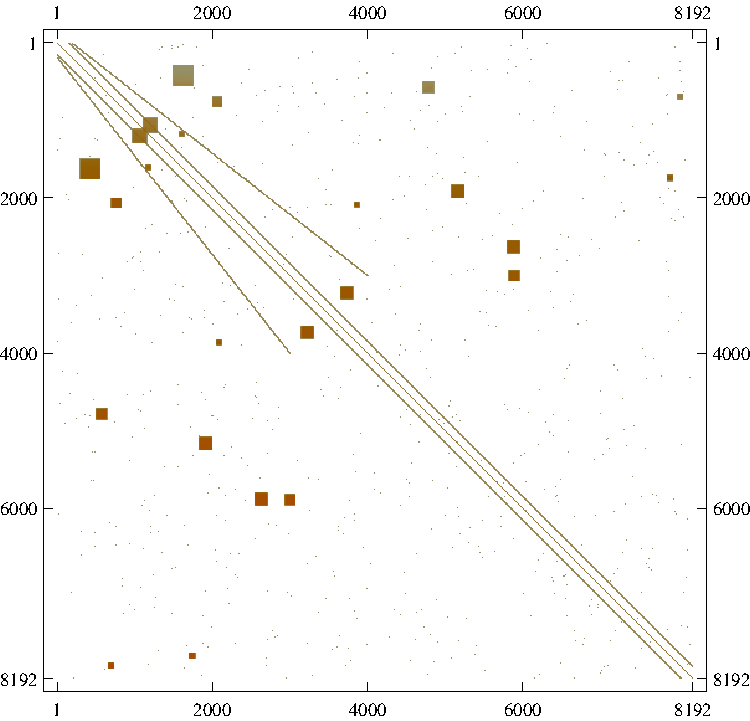
\includegraphics[width=1.0\textwidth]{./images/generated_matrix}
	\caption{Matice vygenerovaná generátorem}
	\label{fig:generatedMtx}
\end{figure}

%\section{Možné optimalizace}
%TODO: popsat moznosti optimalizace - napisu jak by to slo optimalizovat, ale ze jsem to neudelal, protoze mi slo o porovnani mezi % formaty




\section{Měření}

Měření probíhalo na serveru \texttt{star.fit.cvut.cz}.

TODO: popsat jak a kde to budu měřit, cas z omp a cachegrind/callgrind/velikost struktur/pocet uzlu ve strome, zrychleni oproti csr*csr>den, mensi velikost oproti den

\section{Zhodnocení}

